\def \filsti {./Latex/}%\def \filsti {./}%
\documentclass[a4paper]{book}

\usepackage[]{xcolor}
\usepackage{pdfpages}

%% Fix so sections/chapters are manually numbered
\usepackage{tocloft}
\renewcommand\numberline[1]{}
\setcounter{secnumdepth}{0}
%\setcounter{chapter}{0}

% remove "Chapter N" at the start of chapters:
\usepackage{titlesec}
\titleformat{\chapter}[display]
  {\normalfont\bfseries}{}{0pt}{\Huge} 

% shrink margins:
\usepackage[left=2.5cm, right=3cm, bottom=2.5cm, top=2.5cm]{geometry}

% remove "Chapter N" crap in page header/footer
\usepackage{fancyhdr}
\pagestyle{fancy}
\renewcommand{\chaptermark}[1]{\markboth{#1}{}}
\fancyhf{}
\renewcommand{\headrulewidth}{0pt}
\renewcommand{\footrule}{\hbox to \headwidth{\color{blue}\leaders\hrule height \footrulewidth\hfill}}
\renewcommand{\footrulewidth}{1pt}
\fancyfoot[RE]{\tiny\rightmark}
\fancyfoot[LO]{\leftmark}
\fancyfoot[LE,RO]{\thepage}


%% Stop text from indenting
\setlength\parindent{0pt}


%% Graphics are stored in the graphics path
\usepackage{graphicx}
\usepackage{graphbox}
\graphicspath{ {./Latex} }

%% Making hyperlinks in the table of contents
\usepackage{hyperref}
\hypersetup{
    colorlinks,
    citecolor=black,
    filecolor=black,
    linkcolor=blue,
    urlcolor=black
}

\usepackage{titlepic}
\usepackage{datetime2}
\usepackage{tabularray}

%\titlepic{
\includegraphics[scale=0.2]{graphics/jampin.png}}
\title{
\includegraphics[scale=0.2]{graphics/jampin.png}\\ Jammertest 2024 \\ \huge{Test Catalogue}}
\author{Jammertest Consortium}
\date{\today \\ \DTMcurrenttime}

\begin{document}
\maketitle
\SetTblrInner{rowsep=10mm,colsep=10mm}
  \begin{tblr}{
    width=1.8\textwidth,
    stretch = 0,
    colspec = {Q[c,c]cc},
    cell{4}{1}={c=2}{c}
  }
  
\includegraphics[width=50mm, align=c]{graphics/NPRA.png} &
  
\includegraphics[width=50mm, align=c]{graphics/ffi-farger.png}
  \\
  
\includegraphics[width=50mm, align=c]{graphics/norskrom-farger.png} &
  
\includegraphics[width=50mm, align=c]{graphics/nkom-farger.png}
  \\
  
\includegraphics[height=20mm, align=c]{graphics/kartverket-farger.png} &
  
\includegraphics[width=50mm, align=c]{graphics/justervesenet-farger.jpg}
  \\ 
  
\includegraphics[width=50mm, align=c]{graphics/Testnor.png}
  \end{tblr}

\pagebreak

\tableofcontents

\section{Introduction}
Jammertest is a Norwegian government initiative to create a testbed for industry, academia and other authorities to ensure robust and intelligent use of Global Navigation Satellite Systems (GNSS). A testbed is a controlled environment where activities that are not allowed under normal conditions can be carried out safely under control of the authorities. Jammertest is a specific type of testbed where six Norwegian authorities have come together to create an environment where GNSS jamming, spoofing and meaconing is present under controlled conditions in a real world outdoor environment.\newline

This test catalogue describes all centrally planned test cases that can be executed at the Jammertest event at Andøya. For Jammertest, a selected number of tests from this plan will be included in a transmission plan. The transmission plan, which becomes available just before the Jammertest event starts, describes what tests will take place where and at what time. After the Jammertest event the organizers will publish an after the fact transmission log that contains all tests that were run and at what time they were run. The time schedule during the live event will be given in local time, UTC time + 2 (CEST).\newline

A machine readable test catalogue is available in a JSON format, and this (PDF) document is built based on the machine readable test catalouge. The numbering of the tests are (as good as possible) persistant, and will over the years indicate the same tests. New variations of the tests will be given new numbers.

Tests are stacked together in larger test groups and test and varieties of tests are linked to test groups via a numbering system, in such a way that they fulfill this format: TestGroup.Test.TestVariation. Some tests have two numbers, test group and the specific test. Others may have three numbers due to the fact that a specific variation has been added. For example, if power is reduced, a new test variation is created and hence a variation number is added.\newline

Naming of the jammers are linked to the jammer specifications document, that list all jammers with relevant information about the them. See the annexes for this.\newline

This document is auto updated based on changes to the machine readable file, there is no version code apart from the time and date when the document is produced. In the Github repository all produced versions are stored in the history of this file.

\section{Specifications of tests}
Tests are grouped into test groups. Within a test group there is a logical connection between the tests that related to the use case. Hence each test group has a \textit{Rationale} why this is test group is created, that also gives a hint about what to expect when subjected to the specific test. As many tests are on the bleeding edge of GNSS disturbances, the \textit{Rationale} section may be updated between Jammertests based on new knowledge and experiences. \newline

Technical details are stored in the \textit{Test setup} section of the document. The \textit{Areas} section of the document refer to where the test can be run. Here participants need to keep track of in which area they where and this also gives and indication of which areas where the organizers are capable of running the tests. There is also a location out at sea (not numbered) that can be used for maritime related test groups, and a location at the airport in Andenes, for aviation related test groups (only for air planes).

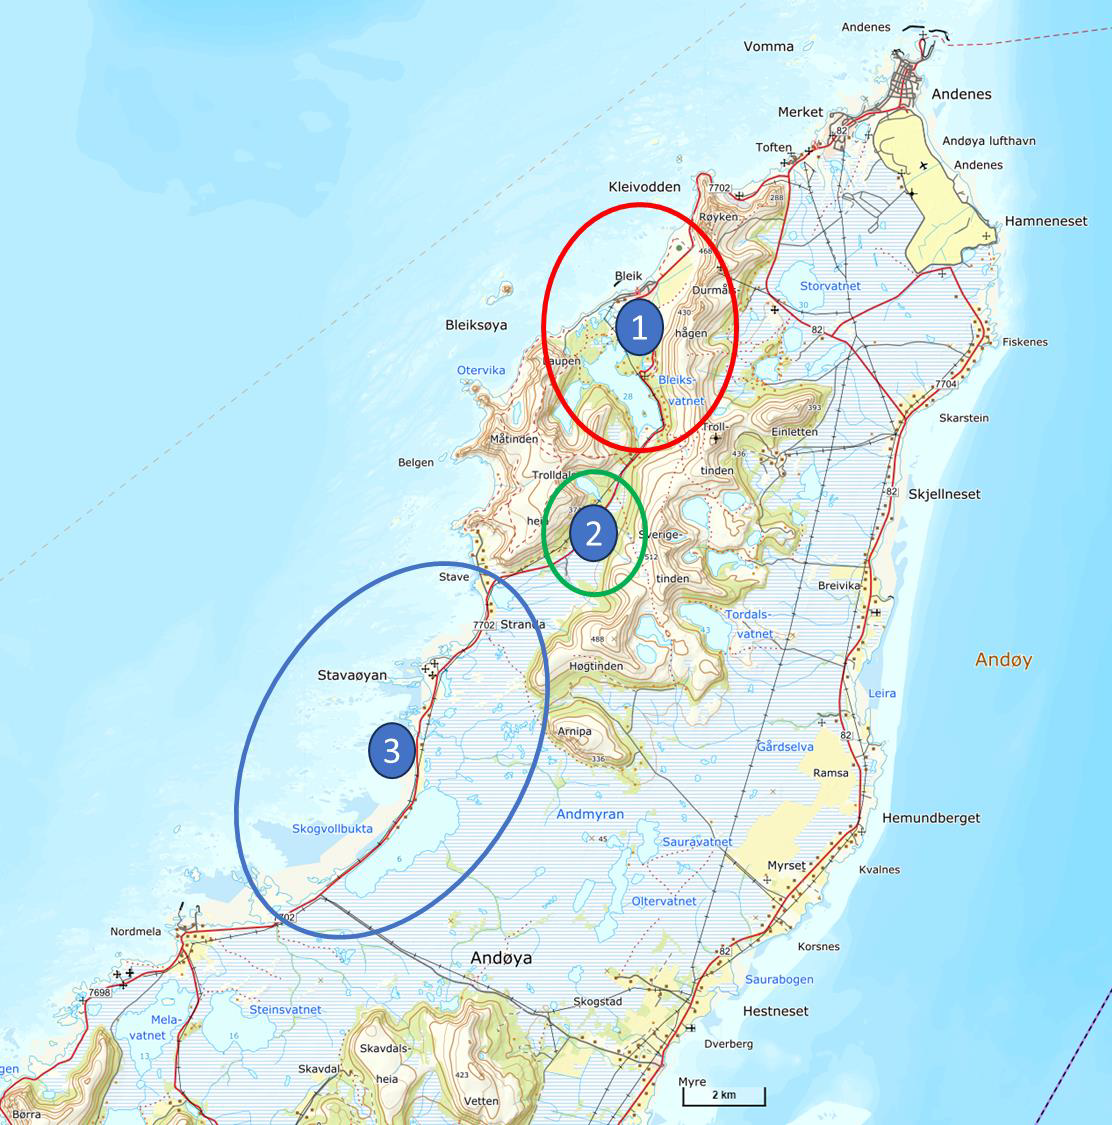
\includegraphics[scale=0.4]{graphics/locations.png}

For each test group a set of tests and test varieties are listed with their unique identification number, a name and a text that describes the test and teh rationale. An approximate power number is also included. If the test is an automated ramp test then the power range is given. A time estimate of how long the test takes to conclude is given in minutes. Between tests there are also grace periods to allow systems to regain normal operation. Grace  times are not given exact as they are dependent on equipment and needs to be discussed with participants beforehand. They also depend on operational concerns. The actual grace time will be calculated from the transmission log after the fact. The location of the transmitter equipment is also given in the test, this is a coarse human readable description of where the transmitting antenna is located. All participants are encouraged to make their own notes on the location of the transmitting antenna if detailed information is needed. There is also a comment field that can be used to document any other relevant information related to the specific test. \newline

For those wanting more information or have feedback about the test group a technical contact is provided for each test group. 

%\chapter{Description of tests}
%Actions
\input{\filsti tests}

%Appendices
\chapter{Appendices}
\section{Appendix A - Description of test areas at Andøya}
\includepdf[pages=-,pagecommand={}]{\filsti appendices/Appendix A - Description of test areas at Andøya.pdf}

\section{Appendix B - GNSS systems overview with signal notation and frequency}
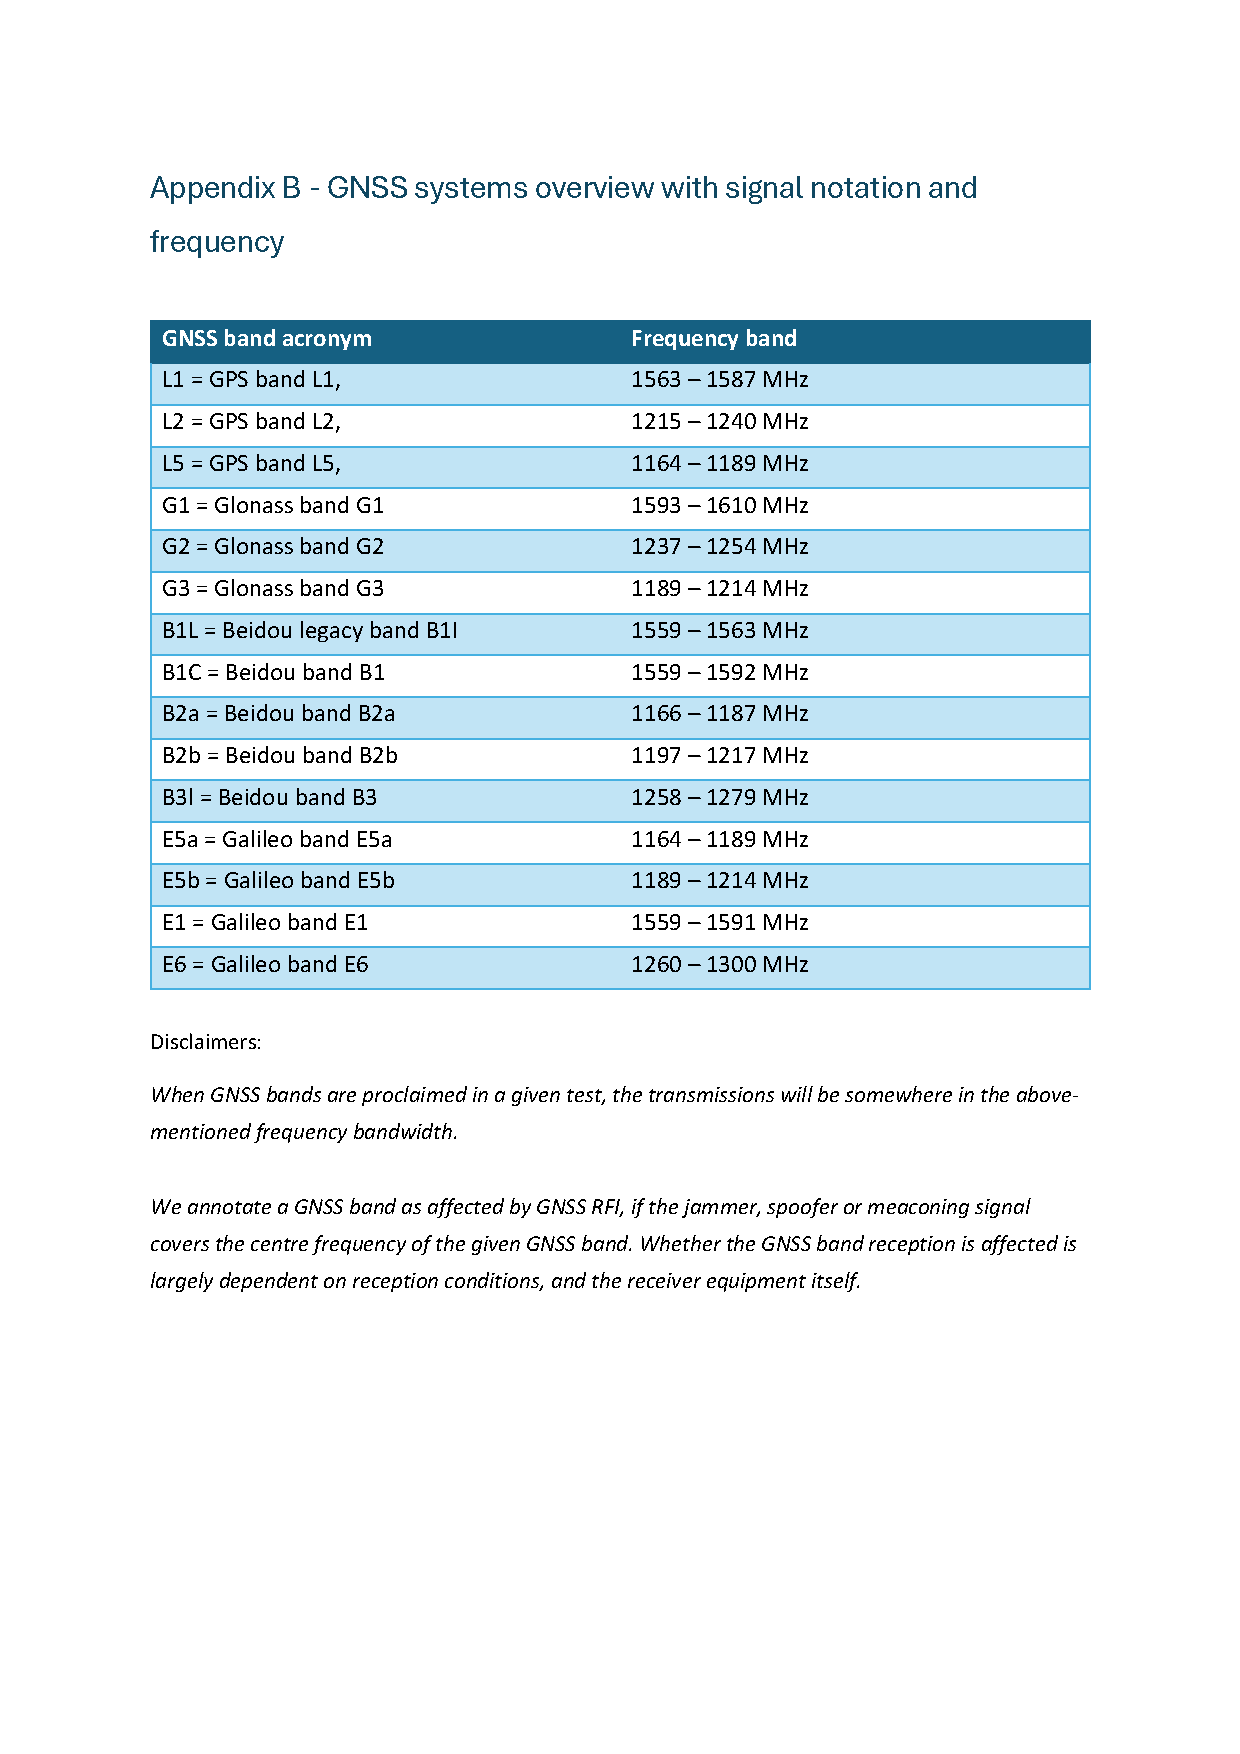
\includepdf[pages=-,pagecommand={}]{\filsti appendices/Appendix B - GNSS systems overview with signal notation and frequency.pdf}

\section{Appendix C - Timing and RF signal distribution at Bleik community house}
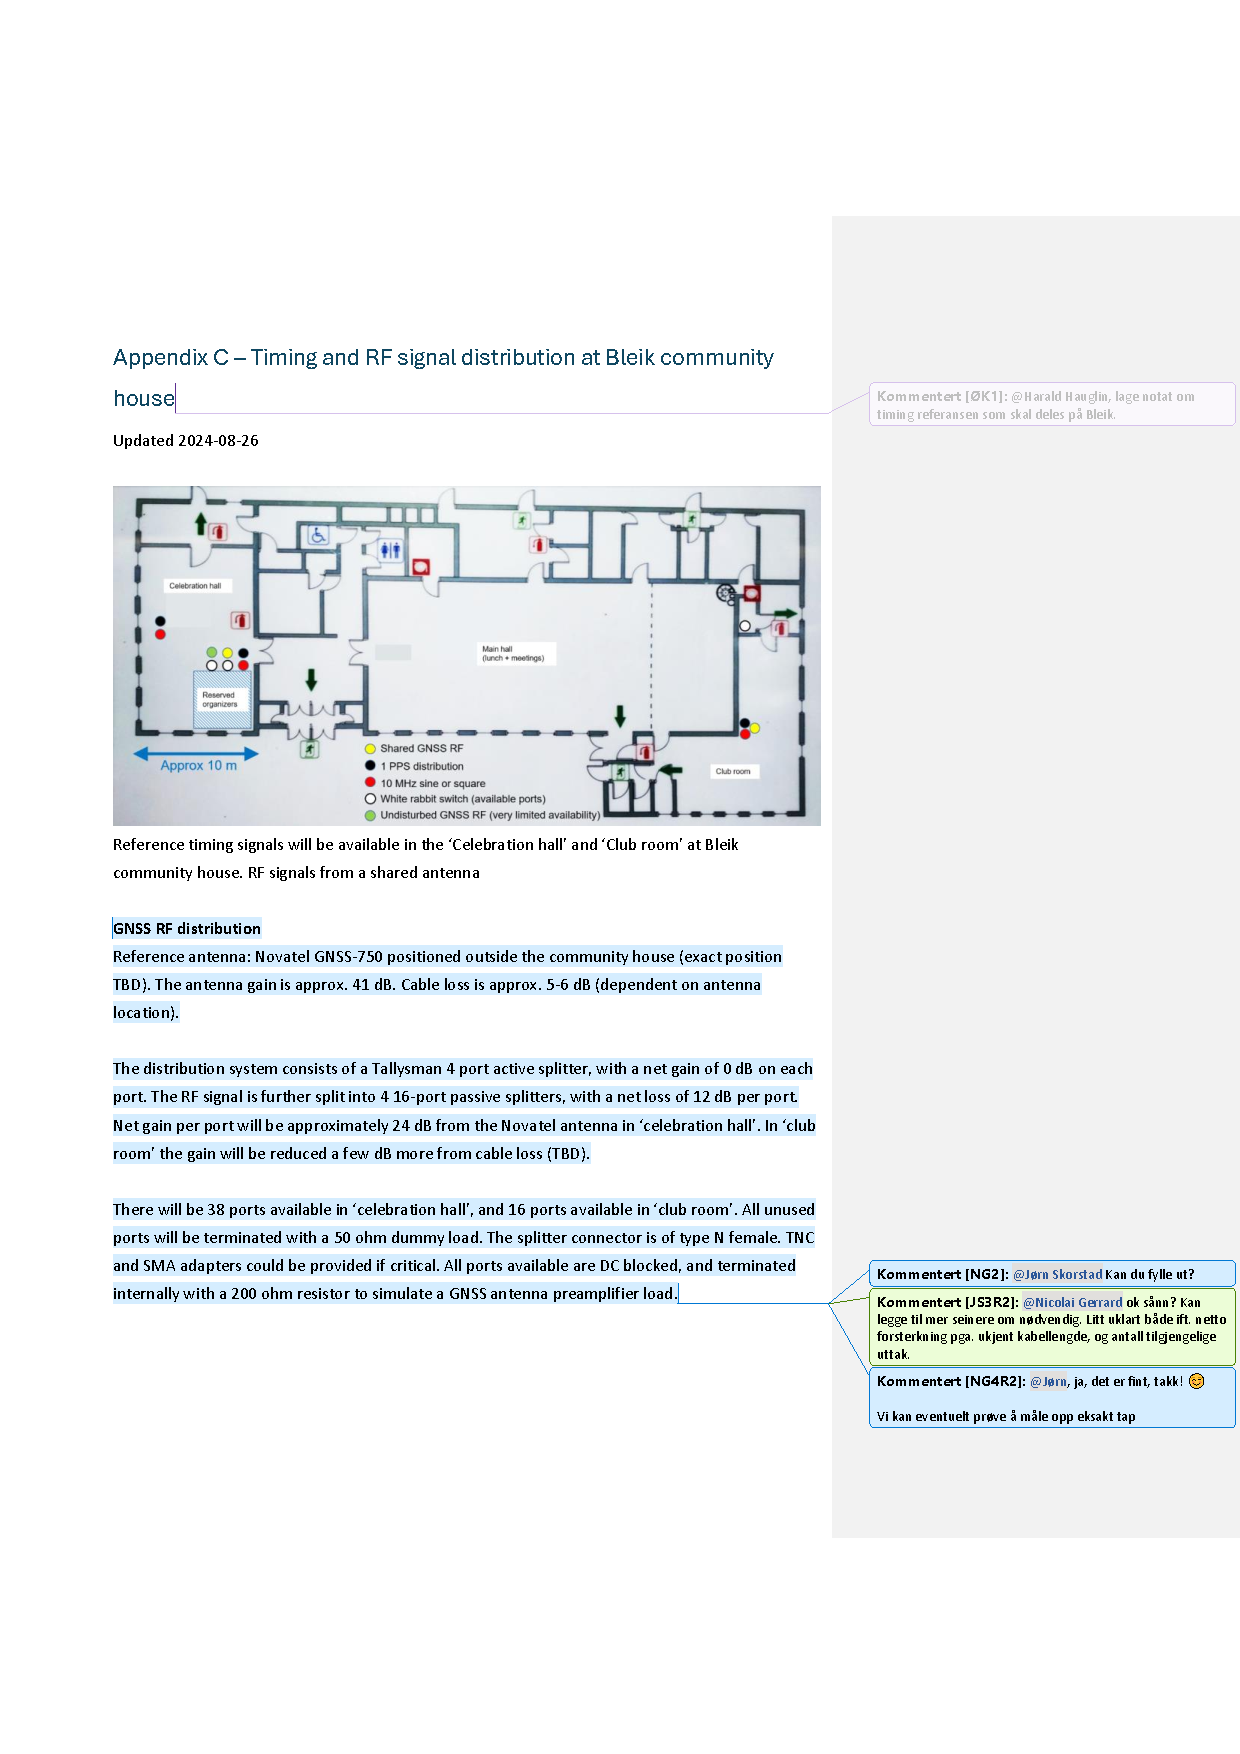
\includepdf[pages=-,pagecommand={}]{\filsti appendices/Appendix C - Timing and RF signal distribution at Bleik community house.pdf}

\section{Appendix D - Overview of inside of Bleik community house}
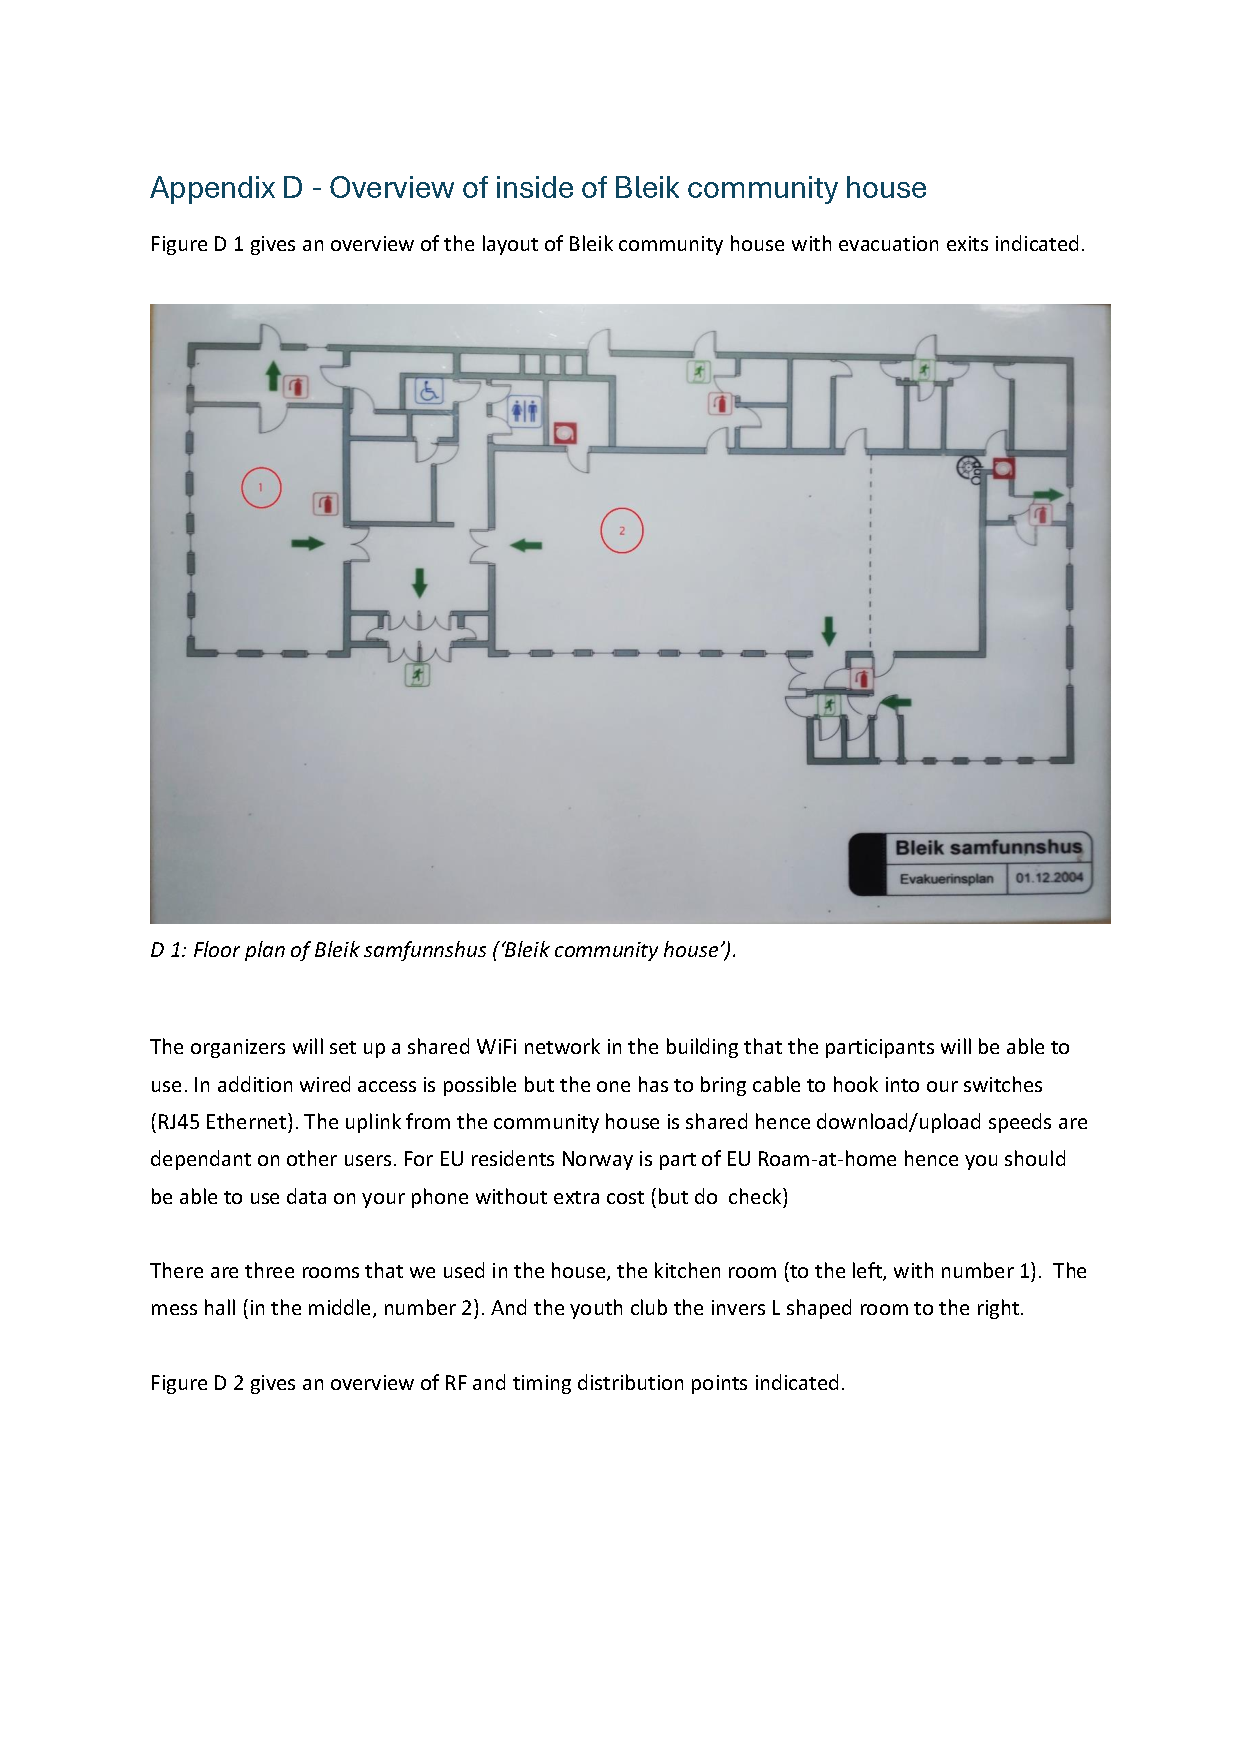
\includepdf[pages=-,pagecommand={}]{\filsti appendices/Appendix D - Overview of inside of Bleik community house.pdf}

\section{Appendix E - Overview of Bleik and HQ}
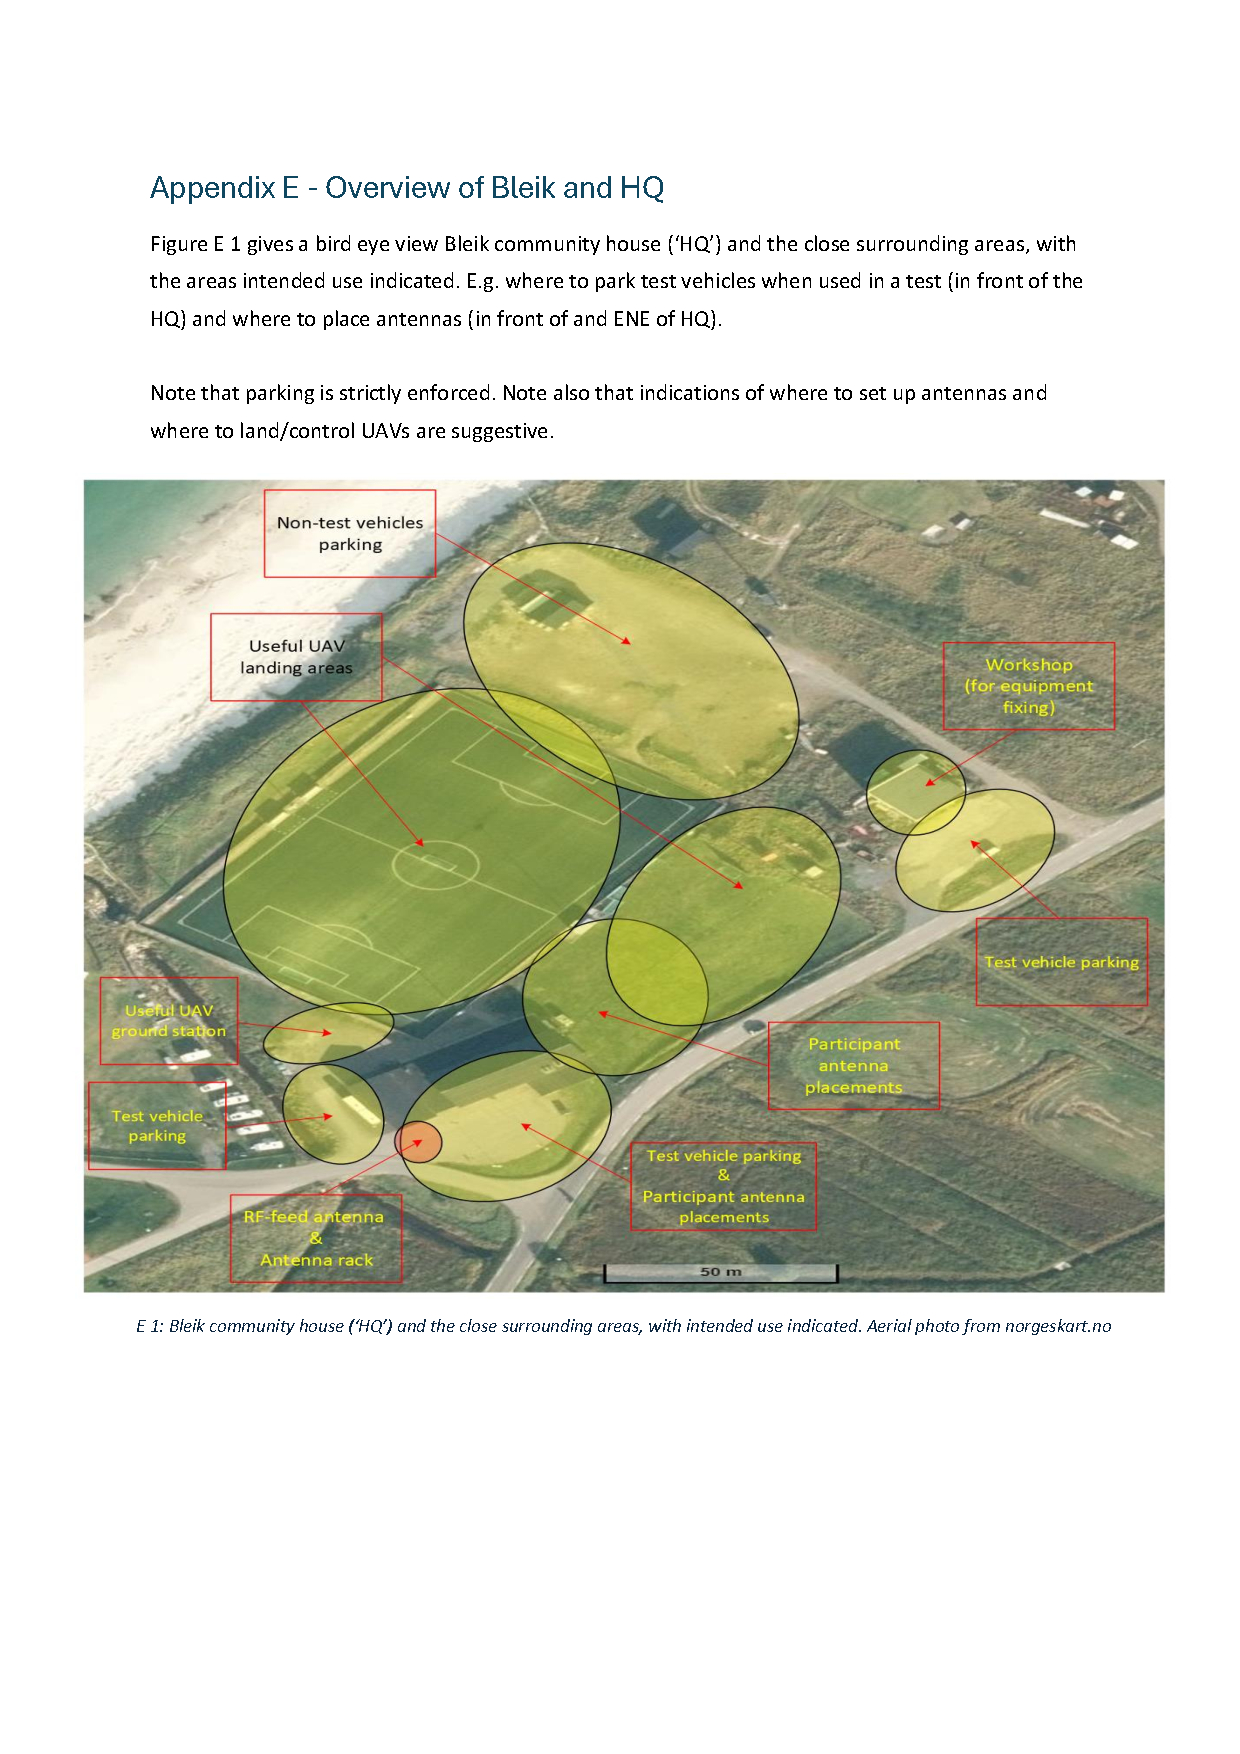
\includepdf[pages=-,pagecommand={}]{\filsti appendices/Appendix E - Overview of Bleik and HQ.pdf}

\section{Appendix F - Overview of spoofed routes}
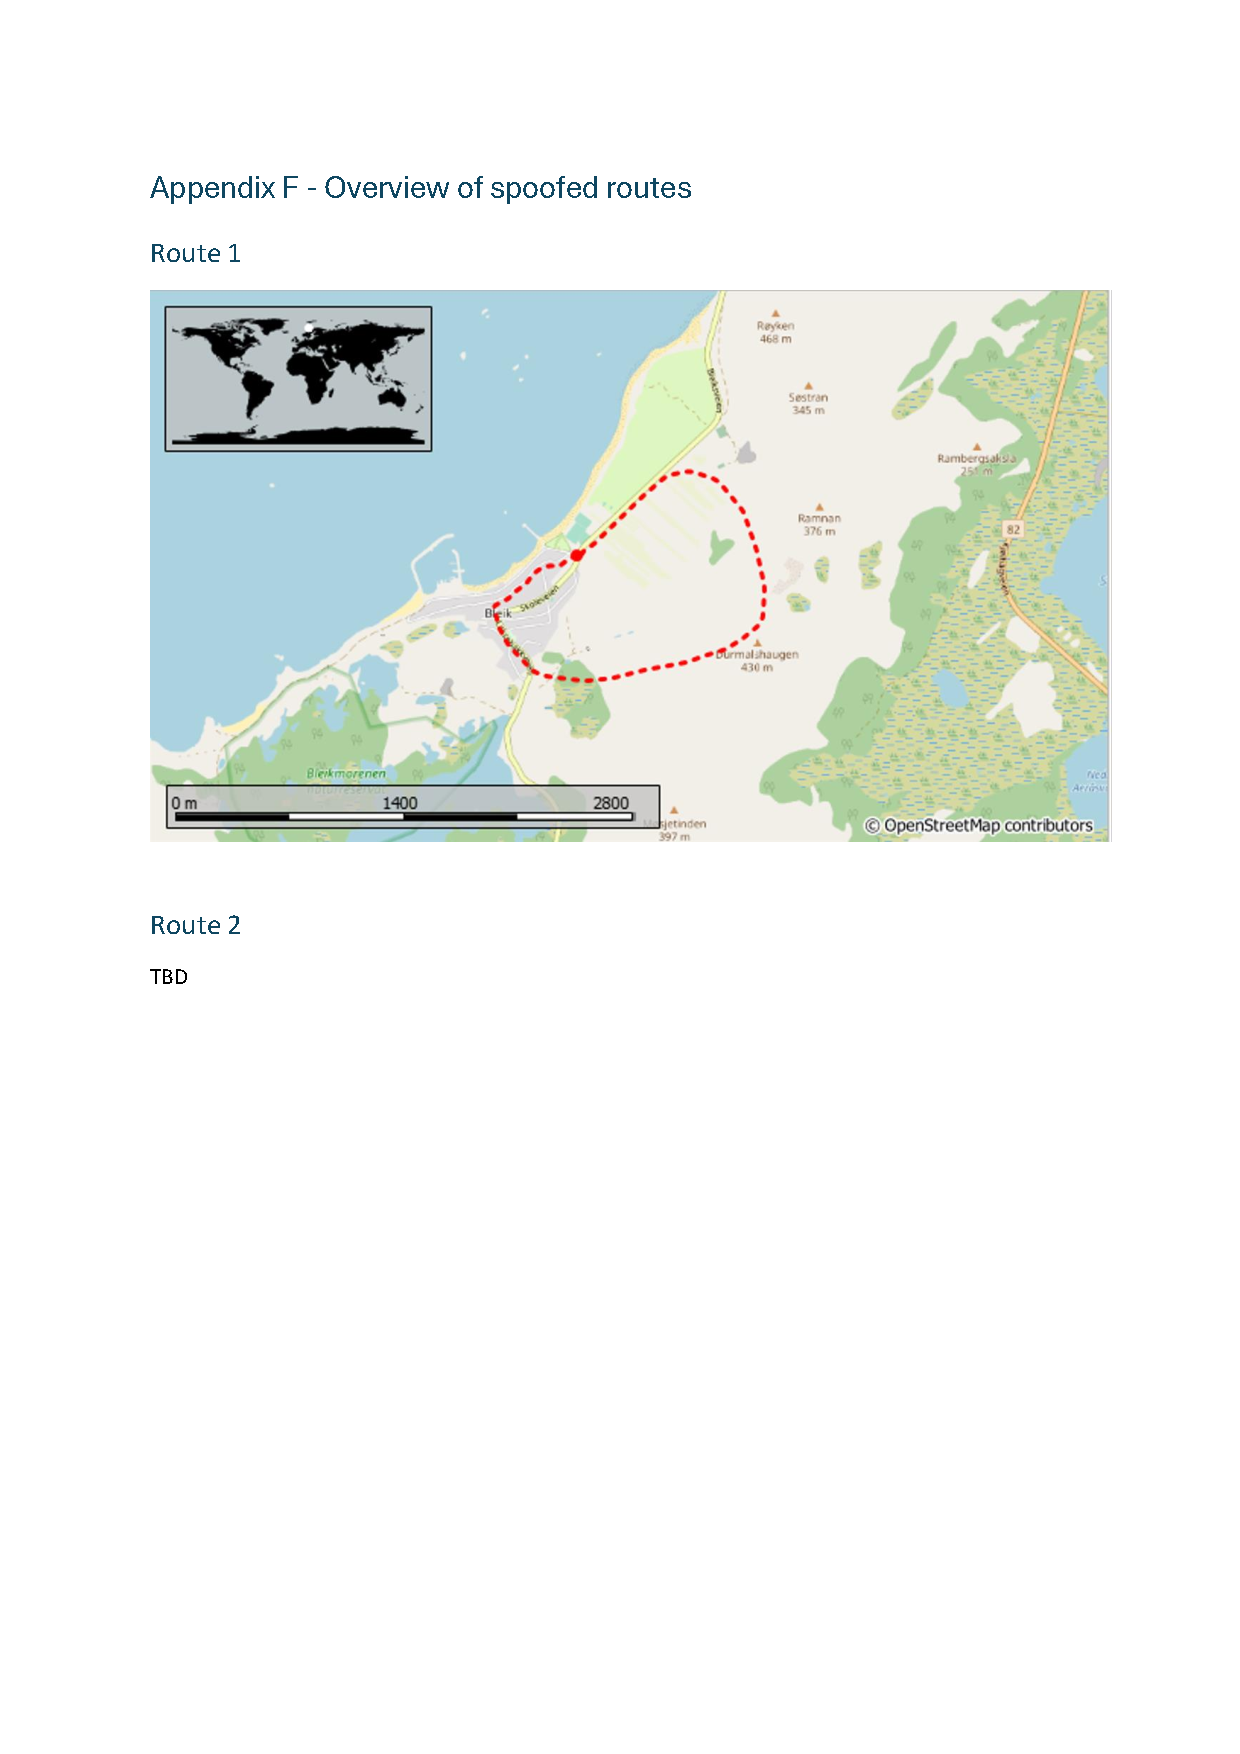
\includepdf[pages=-,pagecommand={}]{\filsti appendices/Appendix F - Overview of spoofed routes.pdf}

\section{Appendix G - Technical details on jammer equipment}
\includepdf[pages={2-},pagecommand={},addtotoc={
    3,subsection,2,Technical details on low-power jammer “S1.1”,p1,
    5,subsection,2,Technical details on low-power jammer “S1.2”,p1,
    7,subsection,2,Technical details on low-power jammer “S1.3”,p1,
    9,subsection,2,Technical details on low-power jammer “S2.1”,p1,
   13,subsection,2,Technical details on low-power jammer “S2.2”,p1,
   17,subsection,2,Technical details on low-power jammer “S2.3”,p1,
   21,subsection,2,Technical details on low-power jammer “S2.4”,p1,
   25,subsection,2,Technical details on low-power jammer “U1.1 to U1.4”,p1,
   26,subsection,2,Technical details on low-power jammer “H1.1”,p1,
   43,subsection,2,Technical details on low-power jammer “H1.2”,p1,
   45,subsection,2,Technical details on low-power jammer “H1.3”,p1,
   46,subsection,2,Technical details on low-power jammer “H1.4”,p1,
   47,subsection,2,Technical details on low-power jammer “H1.5”,p1,
   48,subsection,2,Technical details on low-power jammer “H2.1 and H2.2”,p1,
   49,subsection,2,Technical details on low-power jammer “H3.1”,p1,
   51,subsection,2,Technical details on low-power jammer “H3.2”,p1,
   53,subsection,2,Technical details on low-power jammer “H3.3”,p1,
   59,subsection,2,Technical details on low-power jammer “H4.1”,p1,
   68,subsection,2,Technical details on low-power jammer “H6.1”,p1,
   72,subsection,2,Technical details on low-power jammer “H6.2”,p1,
   79,subsection,2,Technical details on low-power jammer “H6.3”,p1,
   86,subsection,2,Technical details on low-power jammer “H6.4”,p1,
   92,subsection,2,Technical details on low-power jammer “H6.5”,p1,
   98,subsection,2,Technical details on low-power jammer “H6.6”,p1,
  104,subsection,2,Technical details on low-power jammer “F6.1”,p1,
  113,subsection,2,Technical details on low-power jammer “H8.1”,p1,
  115,subsection,2,Technical details on the meaconing setup “Porcellum” / “F1.1”,p1,
  116,subsection,2,Technical details on the high-power jammer “Porcus Major”/ “F8.1”,p1,
  118,subsection,2,Technical details on software defined radio mobile SDR spoofer “F1.2”,p1}]
  {\filsti appendices/Appendix G - Technical details on jammer equipment.pdf}

\section{Appendix H - Andøya ground truth}
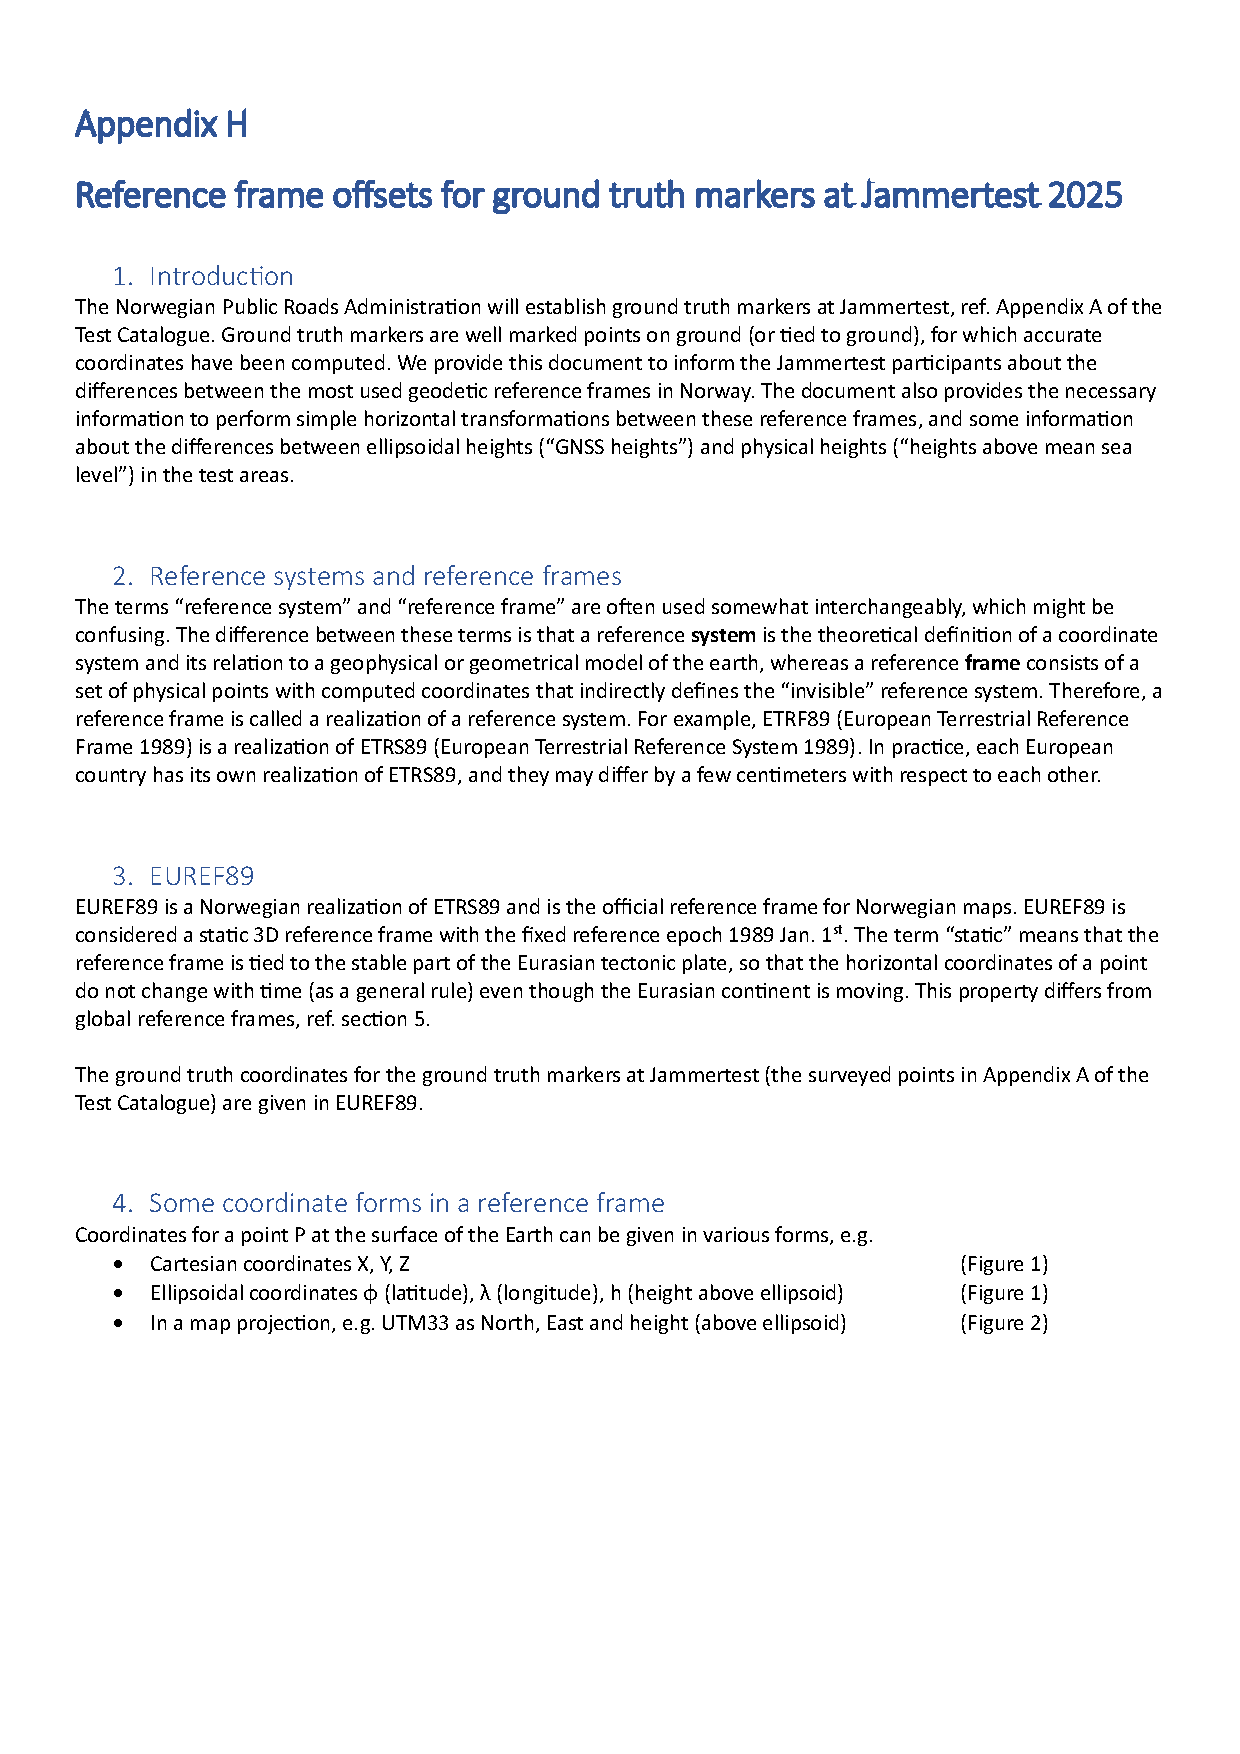
\includepdf[pages=-,pagecommand={}]{\filsti appendices/Appendix H - Andoya_Ground_Truth.pdf}

\end{document}

% Appendix G - Technical details on jammer equipment .......................................................... 2
% Technical details on low-power jammer “S1.1” ................................................................ 3
% Technical details on low-power jammer “S1.2” ................................................................ 5
% Technical details on low-power jammer “S1.3” ................................................................ 7
% Technical details on low-power jammer “S2.1” ................................................................ 9
% Technical details on low-power jammer “S2.2” .............................................................. 13
% Technical details on low-power jammer “S2.3” .............................................................. 17
% Technical details on low-power jammer “S2.4” .............................................................. 21
% Technical details on low-power jammer “U1.1 to U1.4” .................................................. 25
% Technical details on low-power jammer “H1.1”.............................................................. 26
% Technical details on low-power jammer “H1.2”.............................................................. 43
% Technical details on low-power jammer “H1.3”.............................................................. 45
% Technical details on low-power jammer “H1.4”.............................................................. 46
% Technical details on low-power jammer “H1.5”.............................................................. 47
% Technical details on low-power jammer “H2.1 and H2.2” ............................................... 48
% Technical details on low-power jammer “H3.1”.............................................................. 49
% Technical details on low-power jammer “H3.2”.............................................................. 51
% Technical details on low-power jammer “H3.3”.............................................................. 53
% Technical details on low-power jammer “H4.1“ ................................................................. 59
% Technical details on low-power jammer “H6.1”.............................................................. 68
% Technical details on low-power jammer “H6.2”.............................................................. 72
% Technical details on low-power jammer “H6.3”.............................................................. 79
% Technical details on low-power jammer “H6.4”.............................................................. 86
% Technical details on low-power jammer “H6.5”.............................................................. 92
% Technical details on low-power jammer “H6.6”.............................................................. 98
% Technical details on low-power jammer “F6.1” ............................................................ 104
% Technical details on low-power jammer “H8.1“ ............................................................... 113
% Technical details on the meaconing setup “Porcellum” / “F1.1” ................................... 115
% Technical details on the high-power jammer “Porcus Major”/ “F8.1” ............................ 116
% Technical details on software defined radio mobile SDR spoofer “F1.2” ........................ 118Appendices 107

